%! Author = Team Park
%! Date = \today

% Preamble
\documentclass{beamer}

\usetheme{Madrid} % This is a simple and clean theme, but you can change it to other themes like: Berlin, Warsaw, etc.

\title{CNN-Based Classifier for Speech Command Recognition}
\subtitle{A Deep Learning Approach to Audio Classification}
\author{Team Park: D. Hörtenhuber, O. König, W. Laube}
\institute{JKU \\ MLPC}
\date{\today}

\begin{document}

\begin{frame}
  \titlepage
\end{frame}

\begin{frame}{Introduction and Data Preprocessing}
  \begin{itemize}
    \item \textbf{CNN Overview:} CNNs are deep learning models effective in feature extraction from raw data.
    \item \textbf{Data Preprocessing:}
      \begin{itemize}
        \item \textit{Normalization}: Scaling audio data to ensure features are on a similar scale.
        \item \textit{ICA for Noise Reduction}: Applying Independent Component Analysis to reduce background noise and improve signal quality.
      \end{itemize}
  \end{itemize}
\end{frame}

\begin{frame}{CNN Architecture and Training}
  \begin{itemize}
    \item \textbf{CNN Architecture:}
      \begin{itemize}
        \item \textit{Layers}: Four Conv1D layers, each followed by max pooling and dropout layers.
        \item \textit{Filters and Kernel Sizes}: Increasing number of filters and decreasing kernel sizes across layers.
        \item \textit{Dense Layers}: Two dense layers with dropout, leading to the output layer.
      \end{itemize}
    \item \textbf{Training Process:}
      \begin{itemize}
        \item \textit{Data Split}: Training, validation, and test set splits to ensure robust evaluation.
        \item \textit{Optimizer}: Adam optimizer with dropout regularization to prevent overfitting.
      \end{itemize}
  \end{itemize}
\end{frame}

\begin{frame}{Performance Evaluation}
  \begin{itemize}
    \item \textbf{Evaluation Metrics:} Accuracy, precision, recall, F1-score.
    \item \textbf{Results:}
      \begin{itemize}
        \item \textbf{Validation Set:}
          \begin{itemize}
            \item Accuracy: 92.28\%
            \item Precision: 92.75\%
            \item Recall: 92.28\%
            \item F1-score: 92.21\%
          \end{itemize}
        \item \textbf{Comparison with Other Models:}
          \begin{itemize}
            \item Random Forest: Accuracy 89\%
            \item Nearest Neighbour: Pending results
          \end{itemize}
      \end{itemize}
  \end{itemize}
\end{frame}

\begin{frame}{Confusion Matrix and Learning Curves}
  \begin{itemize}
    \item \textbf{Confusion Matrix:}
      \begin{figure}
        \centering
        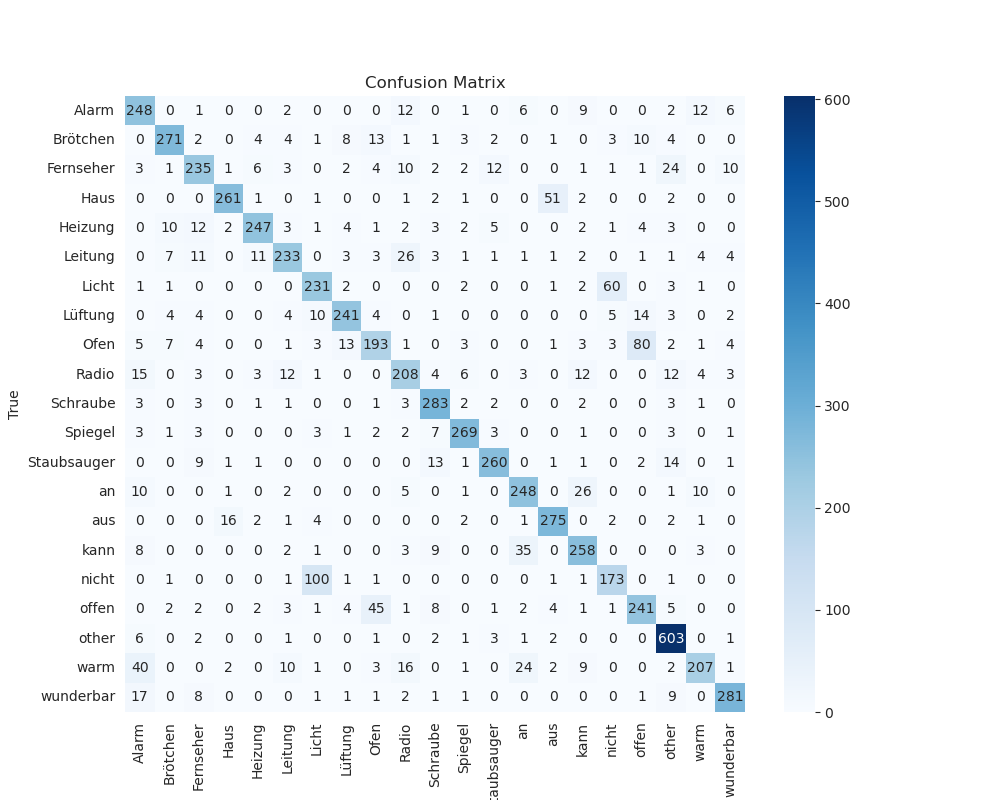
\includegraphics[width=0.8\textwidth]{fig/confusion_matrix.png}
        \caption{Confusion Matrix for 1D CNN}
      \end{figure}
    \item \textbf{Learning Curves:}
      \begin{figure}
        \centering
        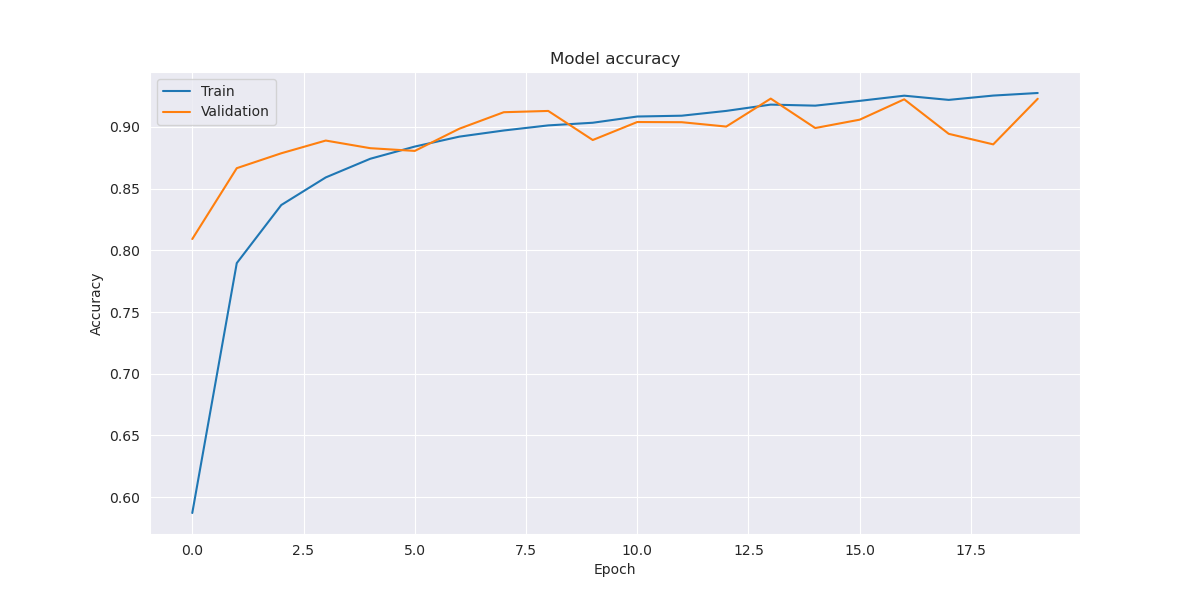
\includegraphics[width=0.8\textwidth]{fig/learning_curves_accuracy.png}
        \caption{Learning Curves for 1D CNN (Accuracy)}
      \end{figure}
  \end{itemize}
\end{frame}

\begin{frame}{Analysis and Conclusion}
  \begin{itemize}
    \item \textbf{Qualitative Analysis:} Performance on realistic scenes, highlighting strengths like noise handling and any observed weaknesses.
    \item \textbf{Conclusion and Future Work:}
      \begin{itemize}
        \item \textit{Summary}: The CNN achieved high accuracy and robustness.
        \item \textit{Future Improvements}: Enhancing the model architecture, experimenting with different preprocessing techniques.
      \end{itemize}
  \end{itemize}
\end{frame}

\end{document}
